% CT-KAT MDPI working manuscript.
% Official class bundle provenance: UPSTREAM.md.
% The journal option "cryptography" is a provisional ACS-format build profile,
% not a submission decision. Replace it after the target journal is confirmed.
\documentclass[cryptography,article,submit,moreauthors]{Definitions/mdpi}

% The 2026 class's submit-mode running head requires 20 pt with current
% fancyhdr.  Setting the documented minimum prevents the header from touching
% the References heading while leaving the upstream class file unmodified.
\setlength{\headheight}{20pt}
\usetikzlibrary{arrows.meta,positioning}
\graphicspath{{figures/}}

\newif\ifNativeResultsAvailable
\NativeResultsAvailablefalse
\newcommand{\NativeAbstractSentence}{Native result summary unavailable.}
\newcommand{\NativeResultSummary}{Native result block unavailable.}
\newcommand{\NativeMeasurementCommit}{\texttt{1aeadb97e0409227aa203ba825a6bfc1d90445bc}}
\newcommand{\NativeHostModel}{not yet imported}
\newcommand{\evidence}[1]{\texttt{#1}}
\newcommand{\toolname}[1]{\textsc{#1}}
% Generated by scripts/render_mdpi_results.py; do not edit.
\NativeResultsAvailablefalse
\renewcommand{\NativeAbstractSentence}{The preregistered native timing campaign is intentionally not summarized in this pre-result draft because its complete, hash-validated named analysis is not yet available.}
\renewcommand{\NativeResultSummary}{The preregistered V10 single-host campaign is still being acquired or validated. No partial, pilot, engineering, or legacy timing value is reported in this draft.}


\firstpage{1}
\makeatletter
\setcounter{page}{\@firstpage}
\makeatother
\pubvolume{1}
\issuenum{1}
\articlenumber{0}
\pubyear{2026}
\copyrightyear{2026}
\datereceived{}
\daterevised{}
\dateaccepted{}
\datepublished{}

\Title{CT-KAT: A Fail-Closed Evidence Pipeline for Constant-Time Risk Screening of Post-Quantum C Implementations}

\Author{Anonymous Authors}
\AuthorNames{Anonymous Authors}
\address{Affiliations are withheld in this anonymized working draft.}
\corres{Correspondence details are withheld in this anonymized working draft.}

\abstract{Constant-time assurance for post-quantum cryptographic software cannot be reduced to functional tests or to a pass from one dynamic tool. We present CT-KAT, an evidence pipeline that combines deterministic correctness gates, generated harnesses, Valgrind-based branch and address observations, a compiler--optimization matrix, assembly-level variable-latency candidates, operand attribution, and controlled timing experiments. Missing correctness, incomplete attribution, invalid controls, and absent artifacts fold to non-clean states rather than being silently ignored. The committed screening corpus contains 25 target--harness pairs and 206 build cells; its reviewed fold records 6 risk-detected, 5 needs-review, 10 inconclusive, and 4 no-finding-observed pairs. A build-matrix and assembly ablation increases the candidate set from 11 pairs in one release build to 22 pairs, quantifying review burden rather than tool accuracy. Frozen KyberSlash variants and Falcon/FN-DSA comparators provide operand-latency and signing-path case studies. \NativeAbstractSentence{} CT-KAT is therefore positioned as an auditable screening and triage system, not as a proof of constant-time behavior.}

\keyword{post-quantum cryptography; constant-time programming; timing side channels; dynamic analysis; KyberSlash; Falcon; reproducibility; artifact evaluation}

\begin{document}

\section{Introduction}
\label{sec:introduction}

Timing side channels have threatened cryptographic implementations since
Kocher showed that execution time can reveal secret information
\citep{kocher96}. Cache behavior, branch prediction, and operand-dependent
instruction latency provide additional channels through which secret-derived
state can affect an observable execution trace \citep{bernstein2005cache}.
Constant-time programming addresses this class of risk by preventing secrets
from controlling branches, memory addresses, and operands of instructions
whose latency varies on the target processor.

The standardization of ML-KEM, ML-DSA, and SLH-DSA in 2024 accelerated the
deployment of post-quantum cryptographic (PQC) C code
\citep{nist2024fips203,nist2024fips204,nist2024fips205}. Functional
known-answer tests (KATs) are necessary in this transition, but they establish
only that selected inputs produce expected outputs. They cannot show that the
computation avoids timing-relevant secret dependence. KyberSlash illustrates
this distinction: on affected compiler--platform combinations, a
secret-derived integer-division operand can produce observable latency even
without a secret-dependent branch or address \citep{bernstein2024kyberslash}.

Available tools expose complementary fragments of this problem. ctgrind-style
Valgrind instrumentation can localize observed secret-dependent branches and
addresses \citep{langley2010ctgrind,nethercote2007valgrind}; dudect compares
timing distributions without locating the responsible instruction
\citep{reparaz2017dude}; assembly inspection can identify candidate
variable-latency instructions without, by itself, establishing that their
operands are secret derived. Moreover, compiler choice and optimization can
change the binary property being tested \citep{simon2018you}. A practical
screening workflow must preserve these boundaries instead of converting every
tool exit code into a binary security label.

This paper presents CT-KAT, a declarative and auditable pipeline for
constant-time risk screening of cryptographic C implementations. CT-KAT does
not introduce a new leakage detector. Its contribution is the controlled
composition of correctness, dynamic structural observations, build-sensitive
evidence, assembly candidates, operand attribution, statistical timing, and
artifact integrity. Every evidence item retains its scope and provenance, and
the fold is fail closed: unavailable or invalid evidence cannot become a clean
claim.

The contributions are as follows:

\begin{enumerate}
\item We define a single-specification workflow that builds a target, verifies
      deterministic correctness, generates analysis harnesses, and records
      structural, build-matrix, assembly, attribution, and timing evidence.
\item We replace an over-broad pass/fail interpretation with four
      claim-scoped evidence states and explicit attribution boundaries. The
      framework never maps a passing dynamic observation to a proof of
      constant-time behavior.
\item We construct versioned evaluation cases for KyberSlash, Falcon and
      prospective FN-DSA comparators, multiple PQC source lineages, and a
      production provider integration. Provenance, correctness, structural
      evidence, and physical timing remain distinct dimensions.
\item We freeze a 28-axis, single-physical-host timing protocol with A/A,
      setup-placebo, positive controls, process repeats, build seals, semantic
      randomness contracts, and deterministic post-analysis. The scope
      explicitly excludes cross-host reproducibility and independent human
      declassification.
\end{enumerate}

The rest of the paper separates the threat model and related work
(Section~\ref{sec:background}) from the pipeline and experimental protocol
(Section~\ref{sec:methods}). Section~\ref{sec:results} reports only evidence
that is admissible in the current artifact state; Section~\ref{sec:discussion}
discusses interpretation and Section~\ref{sec:limitations} states the claim
boundary.

\section{Background and Related Work}
\label{sec:background}

\subsection{Threat Model}

CT-KAT screens three software-level mechanisms. A secret-dependent branch can
alter control flow; a secret-dependent address can alter cache and memory
behavior; and a secret-derived operand to a variable-latency instruction can
alter execution time while leaving branches and addresses unchanged. The
screened attacker observes timing-relevant software execution on the tested
platform. Power, electromagnetic emanations, faults, higher-order leakage,
microarchitectures outside the measured host, and paths not exercised by a
harness are outside the claim.

The unit of evidence is a target, harness, build, and input axis. A source tree
is not called constant time merely because one build or one sampled path has no
finding. The compiled binary and linked inputs are part of the experimental
object.

\begin{table}[H]
\caption{Claim vocabulary used throughout the paper.\label{tab:claim-vocabulary}}
\begin{tabularx}{\textwidth}{LLL}
\toprule
\textbf{State} & \textbf{Meaning} & \textbf{What it does not mean}\\
\midrule
\evidence{risk-detected} & A valid observation crossed the preregistered risk rule. & Universal exploitability or key recovery.\\
\evidence{needs-review} & Valid evidence requires semantic or human attribution. & Safe or vulnerable by default.\\
\evidence{inconclusive} & Correctness, validity, power, attribution, or artifact gates are incomplete. & A negative timing result.\\
\evidence{no-finding-observed} & No risk signal was observed under the recorded build, inputs, host, and protocol. & A constant-time proof.\\
\bottomrule
\end{tabularx}
\end{table}

\subsection{Dynamic Structural Analysis}

ctgrind marks secret bytes undefined for Valgrind/Memcheck and observes whether
the taint reaches executed branch conditions or address calculations
\citep{langley2010ctgrind}. TIMECOP applies related instrumentation at scale,
and MicroWalk records trace differences and leakage magnitude
\citep{bernstein2024report,wichelmann2018microwalk}. These methods provide
useful localization but cover only executed paths and the events modeled by
the backend. An absent warning is therefore an observation, not a proof.

\subsection{Statistical Timing Analysis}

dudect applies Welch's $t$-test to two timing classes and can reveal aggregate
effects from branches, caches, and instruction latency
\citep{reparaz2017dude,gilbert2011testing}. It does not identify the causal
instruction, and its result depends on the input partition, sample size,
environmental noise, and validity of the controls. CT-KAT treats official
dudect as the primary physical timing backend while retaining structural tools
on the same corpus as complementary baselines.

\subsection{Tool Fragmentation and Build Sensitivity}

Prior empirical work reports substantial variation in constant-time tool
coverage and usability \citep{geimer2023systematic}, limited adoption by
cryptographic-library developers \citep{jancar2022they}, and continuing
tooling challenges for PQC signature implementations
\citep{adjonyo2025systematic}. Compiler transformations can also introduce,
remove, or move timing-relevant operations \citep{simon2018you}. CT-KAT
addresses the resulting workflow gap through common configuration,
machine-readable evidence, and a conservative fold rather than by claiming
that one integrated command eliminates the blind spots of its constituent
tools.

\section{Materials and Methods}
\label{sec:methods}

\subsection{System Overview}

One YAML document identifies the source tree, build and KAT commands, target
function, argument roles, secret byte regions, harness templates, compiler
matrix, timing input contract, and reporting policy. CT-KAT first validates
the configuration and expected artifacts. It then builds and executes the KAT,
generates target-specific harnesses, and launches only the enabled evidence
layers. Reports preserve command lines, compiler identity, seeds, input
semantics, hashes, and raw backend outputs.

Figure~\ref{fig:pipeline} shows the current evidence flow. Candidate collection
and interpretation are deliberately separated: an assembly instruction is not
a leak until the relevant operand has adequate attribution, and a timing
statistic is not admissible until its environmental and control gates pass.

\begin{figure}[H]
\begin{adjustwidth}{-\extralength}{0cm}
\centering
\resizebox{\fulllength}{!}{%
\begin{tikzpicture}[
  node distance=7mm,
  stage/.style={draw, rounded corners, align=center, minimum height=13mm,
                minimum width=28mm, fill=gray!6, font=\small},
  arrow/.style={-{Latex[length=2.5mm]}, thick}
]
\node[stage] (spec) {YAML and\\provenance};
\node[stage, right=of spec] (kat) {Build and\\correctness};
\node[stage, right=of kat] (harness) {Generated\\harnesses};
\node[stage, right=of harness] (dynamic) {Structural and\\build matrix};
\node[stage, right=of dynamic] (asm) {Assembly and\\attribution};
\node[stage, right=of asm] (timing) {Controlled\\timing};
\node[stage, right=of timing, fill=gray!15] (fold) {Fail-closed\\evidence fold};
\draw[arrow] (spec) -- (kat);
\draw[arrow] (kat) -- (harness);
\draw[arrow] (harness) -- (dynamic);
\draw[arrow] (dynamic) -- (asm);
\draw[arrow] (asm) -- (timing);
\draw[arrow] (timing) -- (fold);
\end{tikzpicture}}
\end{adjustwidth}
\caption{CT-KAT evidence flow. Later layers add evidence but do not erase an
earlier correctness failure, unresolved attribution, or invalid control.
\label{fig:pipeline}}
\end{figure}

\subsection{Correctness and Harness Generation}

The correctness gate requires a successful build, the declared output
artifacts, and a deterministic KAT or API transcript. A missing or failed
correctness check prevents a clean evidence state because side-channel output
from a functionally wrong binary is not a meaningful security result.

Harness metadata identifies each argument and either a complete secret buffer
or explicit \texttt{secret\_regions}. Region coverage is checked against the
reported object length to prevent accidental under-tainting. Separate generic,
KEM, and signature templates support different API shapes. Structural and
timing experiments use distinct harnesses when their input requirements differ;
the framework does not pretend that one convenient class partition is valid
for every claim.

\subsection{Structural and Build-Matrix Evidence}

The structural layer executes the generated harness under Memcheck and records
observed secret-dependent branches and addresses. The build matrix repeats the
screen across GCC and Clang and optimization levels from \texttt{-O0} through
\texttt{-Os}. A finding that appears in any admissible cell remains visible;
one passing cell cannot declassify it. The matrix records target--harness pairs
and concrete build cells separately so that compiler coverage is not mistaken
for independent implementation diversity.

\subsection{Assembly Candidates and Operand Attribution}

The assembly layer inventories candidate variable-latency operations in each
compiled object. Candidate presence is a build fact. The evidence fold requires
an explicit attribution state---public, secret-derived, mixed, unresolved, or
not applicable---before a stronger interpretation is allowed.

For KyberSlash, CT-KAT also supports a pinned Valgrind/TIMECOP backend patched
to observe tainted variable-latency instruction operands. End-to-end secret-key
taint and direct site-operand seeding are reported separately. This distinction
matters because undefinedness may be lost across recovery, hashing, and
re-encryption boundaries; an empty end-to-end report cannot override direct
site evidence or algorithmic data flow.

\subsection{Fail-Closed Evidence Fold}

The current paper reports the four states in Table~\ref{tab:claim-vocabulary}.
Legacy verdict names remain in compatibility fields but are not treated as a
second source of truth. The fold requires admissible correctness and preserves
structural findings, unresolved candidates, timing validity, review state, and
artifact completeness. In particular, an expired declassification or a raw
timing \texttt{PASS} with insufficient power produces \evidence{inconclusive},
not \evidence{no-finding-observed}.

\subsection{Ground-Truth and Comparator Suites}

\subsubsection{KyberSlash}

The KyberSlash suite pins a PQClean ML-KEM-768 baseline and constructs isolated
KS1, isolated KS2, and combined KS1+KS2 variants. Patch files, upstream
revisions, source hashes, and the three division sites are recorded in a
machine-readable manifest. Eight deterministic full-KEM iterations yield one
byte-identical 37,888-byte transcript across the four modern variants. This
establishes functional equivalence for the frozen test, not general semantic
equivalence or an attack reproduction.

\begin{table}[H]
\caption{Frozen KyberSlash variants and their expected division sites.\label{tab:kyberslash-variants}}
\begin{tabularx}{\textwidth}{LLLL}
\toprule
\textbf{Variant} & \textbf{KS1 \texttt{poly\_tomsg}} & \textbf{KS2 \texttt{poly\_compress}} & \textbf{KS2 \texttt{polyvec\_compress}}\\
\midrule
Stock ML-KEM-768 & absent & absent & absent\\
KS1 only & present & absent & absent\\
KS2 only & absent & present & present\\
KS1+KS2 & present & present & present\\
Historical Kyber & present & present & present\\
\bottomrule
\end{tabularx}
\end{table}

The physical campaign uses two distinct views. Full-KEM chosen-ciphertext axes
hold one key fixed and vary public ciphertext pools. Three vulnerable/patched
site pairs separately exercise operand bins under exact linked-binary
contracts. The former is a public-input contrast; the latter is a
hardware-latency canary. Neither is labeled a full key-recovery experiment.

\subsubsection{Falcon and Prospective FN-DSA}

The Falcon comparator pins PQClean reference implementations and c-fn-dsa at
degrees 512 and 1024. For c-fn-dsa, a native floating-point profile and an
integer floating-point-representation (FPR) profile are compiled under
different exact flag contracts. Seeded key generation and signing produce
byte-identical transcripts between the c-fn-dsa profiles at each degree.
Reference Falcon and c-fn-dsa are not assumed to produce identical encodings,
and c-fn-dsa is described as a prospective comparator rather than evidence of
FIPS 206 conformance.

\begin{table}[H]
\caption{Falcon/FN-DSA comparator scope. Structural findings remain study inputs until their recorded attribution and physical timing are complete.\label{tab:falcon-scope}}
\begin{tabularx}{\textwidth}{LLLL}
\toprule
\textbf{Source} & \textbf{Degrees} & \textbf{Profiles} & \textbf{Timed boundary}\\
\midrule
PQClean Falcon reference & 512, 1024 & reference implementation & full signature API\\
c-fn-dsa & 512, 1024 & native FP; integer FPR & seeded full signature API\\
\bottomrule
\end{tabularx}
\end{table}

Full-signature timing includes key decoding, sampler behavior, rejection, and
variable-length or padded encoding as implemented by each target. Output-length
association is therefore analyzed as a secondary endpoint and cannot erase a
primary timing finding.

\subsection{Source and Build Diversity}

The source/build corpus distinguishes primary upstream lineages from parameter
sets, compiler cells, architecture profiles, and integrations. PQClean,
c-fn-dsa, mlkem-native, and mldsa-native are maintained as four primary
upstream lineages. The count does not imply four from-scratch implementations:
shared ancestry is recorded and its fraction is unmeasured. OpenSSL 3.5 is a
production provider-API integration and is not counted as a fifth lineage.

\begin{table}[H]
\caption{Source/build diversity dimensions. Timing evidence is not inferred from build or KAT evidence.\label{tab:lineages}}
\begin{tabularx}{\textwidth}{LLLL}
\toprule
\textbf{Source} & \textbf{Role} & \textbf{Algorithms} & \textbf{Boundary}\\
\midrule
PQClean & screening/reference lineage & ML-KEM, ML-DSA, SLH-DSA, Falcon & exact imported trees\\
c-fn-dsa & prospective comparator lineage & Falcon/FN-DSA & no final FIPS 206 conformance claim\\
mlkem-native & separately maintained native package & ML-KEM-512/768/1024 & portable and architecture-native builds\\
mldsa-native & separately maintained beta package & ML-DSA-44/65/87 & beta API; portable and architecture-native builds\\
OpenSSL 3.5 & provider integration & ML-KEM and ML-DSA APIs & not an independent lineage\\
\bottomrule
\end{tabularx}
\end{table}

The frozen build contract covers x86\_64 and AArch64, GCC and Clang, portable
and architecture-native profiles, five optimization settings, deterministic
smoke transcripts, KAT digests, machine headers, linked native symbols, and
architecture instruction markers. These checks establish provenance, build,
and equivalence evidence only. They do not substitute for physical timing on
either architecture.

\subsection{Preregistered V10 Native Timing Protocol}
\label{sec:timing-protocol}

The final campaign is bound to CT-KAT commit
\texttt{\seqsplit{1aeadb97e0409227aa203ba825a6bfc1d90445bc}}. It requires one
non-virtualized physical x86\_64 Linux host, one pinned logical CPU, the
\texttt{performance} governor, simultaneous multithreading disabled, and turbo
disabled. Host, boot, CPU, compiler executable, binary, source, configuration,
and linked-input identities are recorded. The one-host design supports
host-scoped evidence only.

Before any final sample, two complete blocker-free control rehearsals at the
same commit are combined into a machine-validated qualification. They are
operational repetitions, not independent inferential replicates. The final
runner rejects pilot reuse, final resume, dirty worktrees, changed manifests,
and absent qualification.

The campaign contains four components, 26 target executions, and 28 primary
axes. Each axis uses three process repeats, pre-generated input pools, a common
timed API boundary, warm-up, fixed seeds, and predeclared stopping and
exclusion rules. Non-operand KEM and signature harnesses read both class pools
and use a masked selection into shared work buffers before timing. Semantic
randomness contracts are explicit even when an implementation has no
\texttt{randombytes} header. Operand canaries and c-fn-dsa use seeded
interposition; KyberSlash operand timing requires zero random-number calls in
the measured interval.

The control ladder includes A/A, setup-placebo, and positive controls. A raw
dudect status is admissible only if the target and controls pass the frozen
validity checks. Official dudect supplies primary physical timing evidence;
TIMECOP and MicroWalk are executed on the same corpus as complementary
baselines. Every final timing harness emits a pre-measurement build seal.

% Generated by scripts/render_mdpi_results.py; do not edit.
\begin{table}[H]
\caption{Fail-closed states in the committed screening corpus. Counts refer to target--harness pairs and must not be interpreted as an accuracy rate.\label{tab:corpus-states}}
\begin{tabularx}{\textwidth}{Lr}
\toprule
\textbf{Evidence state} & \textbf{Pairs}\\
\midrule
\texttt{risk-detected} & 6\\
\texttt{needs-review} & 5\\
\texttt{inconclusive} & 10\\
\texttt{no-finding-observed} & 4\\
\bottomrule
\end{tabularx}
\end{table}

\begin{table}[H]
\caption{Candidate-generation ablation. The first three rows measure review burden, not detection accuracy; only the reviewed fold emits final evidence states.\label{tab:ablation}}
\begin{tabularx}{\textwidth}{Lrrrr}
\toprule
\textbf{Stage} & \textbf{Cells} & \textbf{CT findings} & \textbf{Asm candidates} & \textbf{Candidate pairs}\\
\midrule
Single release build & 24 & 11 & 0 & 11\\
Full compiler/flag matrix & 206 & 13 & 0 & 13\\
Matrix plus assembly scan & 206 & 13 & 16 & 22\\
Reviewed fail-closed fold & 206 & 13 & 16 & --\\
\bottomrule
\end{tabularx}
\end{table}

\begin{table}[H]
\caption{Frozen V10 native timing scope. Target executions are component-local and are not counts of independent implementations.\label{tab:v10-scope}}
\begin{tabularx}{\textwidth}{Lrrr}
\toprule
\textbf{Component} & \textbf{Targets} & \textbf{Axes} & \textbf{Protocol rows}\\
\midrule
\texttt{committed-corpus-refresh} & 6 & 8 & 2,220,000\\
\texttt{kyberslash-contrast} & 10 & 10 & 3,300,000\\
\texttt{falcon-contrast} & 6 & 6 & 1,530,000\\
\texttt{diverse-lineages} & 4 & 4 & 1,170,000\\
\midrule
Total & 26 & 28 & 8,220,000\\
\bottomrule
\end{tabularx}
\end{table}


\subsection{Deterministic Analysis Policy}

Each component, target, harness, and semantic axis remains a separate primary
result. A valid official-dudect \texttt{FAIL} maps to
\evidence{risk-detected}; a valid \texttt{WARNING} maps to
\evidence{needs-review}; invalid or confounded evidence maps to
\evidence{inconclusive}; and a valid \texttt{PASS} maps to
\evidence{no-finding-observed} under the host and protocol.

Predeclared secondary comparisons use a two-sided Welch test over the three
per-process class-mean deltas, with Holm adjustment within each comparison
family. Falcon output-length association reports ordinary and within-class
centered Pearson analyses. Secondary analyses cannot declassify a primary
finding. The named analyzer writes deterministic JSON, CSV, and Markdown;
re-running in check mode must reproduce identical bytes.

\subsection{Artifact Integrity and Promotion}

All four component reports, three same-corpus baselines, assembly evidence,
control qualification, host hash manifest, and named analysis are indexed by a
schema-v5 single-host bundle. Missing targets, controls, repeats, build seals,
randomness contracts, or hashes abort analysis. Automatic corpus mutation is
disabled. Independent human review and a second physical host are optional
follow-up evidence and are not represented as completed gates in this paper.

\subsection{Use of Generative AI Assistance}

A generative AI coding assistant was used to help restructure the working
manuscript, draft prose, and implement documentation and test scaffolding. The
authors are responsible for checking every claim against the versioned source
and machine-readable artifacts, for reviewing all generated text and code, and
for the final submitted manuscript. The assistant did not create or alter V10
measurement observations.

\section{Results}
\label{sec:results}

\subsection{Committed Screening Corpus}

The committed corpus contains 25 target--harness pairs. Correctness is recorded
as passing for 21 pairs and not run for four synthetic pairs. The fail-closed
fold produces 6 \evidence{risk-detected}, 5 \evidence{needs-review}, 10
\evidence{inconclusive}, and 4 \evidence{no-finding-observed} pairs
(Table~\ref{tab:corpus-states}). These counts describe the state of a
heterogeneous screening corpus; combining them into sensitivity, specificity,
or accuracy would require an independent and consistently labeled oracle that
the corpus does not provide.

The result differs materially from the older nine-class narrative. The three
ML-DSA signing pairs and the SLH-DSA pair are inconclusive because prior
declassification was withdrawn: rejected signing iterations can retain
secret-derived state, and the exact-build raw probe needed for the older
public-output explanation was not preserved. Falcon reference and c-fn-dsa
structural findings remain unresolved or pending. CT-KAT therefore does not
describe these implementations as accepted variable time.

\subsection{Build and Assembly Ablation}

A single release-build structural screen identifies 11 candidate pairs among
24 evaluated pairs. Expanding to the complete compiler/optimization matrix
identifies 13 candidate pairs across 206 build cells and exposes two
build-sensitive pairs. Adding assembly candidates raises the review set to 22
pairs, with candidate instructions in 16 pairs
(Table~\ref{tab:ablation}). These increments quantify candidate-generation
coverage and analyst burden. They are not false-positive or accuracy rates.

The reviewed fold includes one additional pair and reports final evidence
states only where correctness, attribution, and review fields permit it. This
separation prevents a large candidate count from being presented as a large
number of confirmed leaks.

\subsection{KyberSlash Static and Ground-Truth Evidence}

The stock and three patched-in KyberSlash variants pass the frozen deterministic
full-KEM transcript check. Ordinary branch/address Memcheck records no finding
for those four modern variants, matching the expected blind spot for
operand-latency leakage. The assembly matrix locates the expected surviving
division functions according to the variant. Direct site-operand attribution
identifies all expected KS1 and KS2 sites with the pinned backend.

The historical Kyber source additionally has a compiler-induced branch in
\path{poly_frommsg} in selected Clang cells. That branch is recorded as a
separate build-sensitive structural finding and is not mislabeled as a
KyberSlash division. Full-KEM and operand-bin physical contrasts remain in the
V10 result block below.

\subsection{Falcon Comparator Evidence}

Both Falcon degrees have exact imported-source hashes and explicit secret-key
regions. The c-fn-dsa native-FP and integer-FPR profiles produce matching
seeded transcripts within each degree. Structural observations cover encoded
key decoding, private-key completion, sampling, signing acceptance, and
signature encoding. Floating-point opcode inventories and exception probes are
build and deterministic-KAT evidence; absence of a floating-point exception in
the probe is not generalized to all keys.

No static observation is promoted to a timing or standards-conformance claim.
The six full-signature physical axes and output-length secondary analysis are
reserved for the validated V10 analysis.

\subsection{Diverse Upstream and Integration Evidence}

The source/build manifest records four primary upstream lineages and one
OpenSSL provider integration. mlkem-native and mldsa-native have pinned releases,
revisions, tree hashes, algorithm parameters, KAT digests, portable/native
profiles, and x86\_64/AArch64 contracts. Shared-code ancestry remains
unmeasured, and the independent-review packets remain pending; consequently,
the result is stated as provenance and build coverage, not four independent
implementations or architecture-general timing evidence.

\subsection{V10 Single-Host Native Timing}
\label{sec:native-results}

\NativeResultSummary{}

% Generated by scripts/render_mdpi_results.py; do not edit.
\begin{table}[H]
\caption{Reserved location for the 28-axis V10 native timing analysis. This table will be generated only from a complete, hash-validated schema-v5 bundle.\label{tab:native-results}}
\begin{tabularx}{\textwidth}{L}
\toprule
\textbf{Pre-result state}\\
\midrule
\texttt{NATIVE-RESULTS-PENDING}: final values intentionally withheld until deterministic named analysis passes all validators.\\
\bottomrule
\end{tabularx}
\end{table}


\ifNativeResultsAvailable
All 28 primary axes passed their frozen timing-validity gates. The three
\evidence{risk-detected} rows are the PQClean, mlkem-native portable, and
mlkem-native x86\_64 ML-KEM decapsulation \texttt{valid\_tuple} axes. Each
class changes a matching secret key, ciphertext, and the public material
embedded in the secret key together. These are therefore reproducible mixed
input timing signals on this host, not secret-key-only leakage attribution or
key-recovery evidence. The distinct PQClean ciphertext-only, FO-path, and
KyberSlash chosen-ciphertext axes remain \evidence{no-finding-observed} under
their own input contracts.

Exactly one of 17 preregistered pairwise comparisons is Holm-significant: the
mlkem-native portable versus x86\_64 \texttt{valid\_tuple} class-mean-delta
contrast ($p_{\mathrm{Holm}}=0.000288$). Both profiles retain a primary
\evidence{risk-detected} state, so this secondary result compares signal
magnitude and does not rank either profile as secure. None of the six Falcon,
six KyberSlash chosen-ciphertext, three KyberSlash operand, or one ML-DSA
pairwise comparisons is Holm-significant.

Three of 13 signature-length endpoints are variable-length PQClean Falcon
outputs. Their largest absolute within-class Pearson coefficient is below
$0.0024$; the remaining ten endpoints are fixed length. The length analysis
does not declassify the primary signature results.
\else
No native interpretation is emitted until every value can be generated from a
complete \path{paper_native_analysis.json}. Preliminary or partial statistics
are not copied from the legacy WISA manuscript.
\fi

\section{Discussion}
\label{sec:discussion}

\subsection{Why Evidence Composition Matters}

The static corpus demonstrates that additional layers expand the review set,
not that they monotonically increase an abstract accuracy score. The build
matrix exposes compiler-sensitive observations, while the assembly layer
surfaces candidates outside branch/address models. Correctness and attribution
then determine which signals are interpretable. A fail-closed fold is useful
because missing evidence remains visible instead of being collapsed into a
pass.

KyberSlash is the clearest example of the complementary design. Ordinary
Memcheck can remain quiet while a division with a secret-derived operand
survives in the compiled binary. Assembly presence alone still lacks operand
provenance, and direct operand attribution still does not establish an
end-to-end remotely exploitable timing channel. The V10 full-KEM and operand
canaries occupy those distinct claim scopes rather than being merged into one
label. On the measured Intel host, all KyberSlash primary axes and all three
vulnerable-versus-patched operand comparisons produced no timing finding under
the frozen protocol. This negative physical observation does not erase the
known division sites or their direct operand attribution; it limits what was
observable on this processor and input partition.

\subsection{Interpretation of Timing States}

The physical result is conditional on one CPU, one operating-system and
compiler stack, the frozen binaries, the declared input distributions, and the
control protocol. A valid \texttt{FAIL} establishes a reproducible risk signal
under those conditions. A valid \texttt{PASS} states only that the campaign did
not observe a signal above its decision rule. An invalid control is not rescued
by a small target statistic.

Three process repeats estimate within-host stability but do not create three
independent machines. Likewise, a comparison between portable and native
profiles on one x86\_64 host does not establish AArch64 behavior. These
distinctions are retained in the generated tables and the final artifact
metadata.

\subsection{Implications for PQC Engineering}

CT-KAT is most useful as an early and repeatable screen in a larger assurance
process. It can prevent functionally incorrect targets, changed binaries,
unreviewed assembly candidates, and invalid timing environments from receiving
clean labels. It can also direct a reviewer toward exact build cells and
functions. Formal verification, leakage-resilient design, power and
electromagnetic evaluation, fault analysis, and attack-specific validation
remain separate activities.

The framework also makes deployment identity explicit. A report about a
portable reference build does not automatically describe a native backend or
an OpenSSL provider. Treating source, profile, compiler, linked binary, and
integration as separate coordinates is more verbose than one verdict, but it
is necessary for reproducible binary-level claims.

\subsection{Responsible Interpretation}

The KyberSlash cases are intended to reproduce and attribute known software
mechanisms and controlled latency canaries. This paper does not claim new key
recovery, provide a generalized exploitation recipe, or infer vulnerability
for implementations outside the pinned sources and builds. Raw artifacts are
preserved for scientific review, while paper wording remains limited to the
predeclared evidence scope.

\section{Limitations}
\label{sec:limitations}

Dynamic observations cover only executed paths and modeled events. Harness
input distributions may omit rare behavior. Assembly scanning is limited to
its candidate instruction model, and semantic attribution can require human
review. Compilers and processors outside the frozen matrices can transform or
execute the same source differently.

The final physical campaign uses one x86\_64 host. It does not establish
cross-host reproducibility, architecture generality, or independent analyst
agreement. Human review packets are machine-readable but have no completed
two-person sign-off in the current campaign. These absences are limitations,
not silently relaxed gates.

The Falcon comparison includes reference Falcon and a pinned prospective
c-fn-dsa implementation. It does not establish final FIPS 206 conformance.
mldsa-native uses a beta release. OpenSSL contributes integration evidence but
not a distinct implementation lineage. Shared ancestry among upstreams is
recorded but not quantitatively bounded.

CT-KAT currently executes on desktop Linux. A Cortex-M4 binary can in principle
be cross-compiled on the desktop and inspected, but architecture-specific ARM
disassembly, instruction-latency models, symbol attribution, and binary/harness
contracts are required before this becomes an implemented backend. Connecting
an M4 board does not make x86 Valgrind execute ARM instructions, and on-device
timing would be a separate campaign. No M4 execution result is claimed here.

Finally, CT-KAT does not analyze power, electromagnetic, fault, or higher-order
masked leakage. Configuration files invoke build and test commands and must be
reviewed before use on untrusted projects.

\section{Conclusions}
\label{sec:conclusions}

CT-KAT turns fragmented constant-time checks into an auditable, fail-closed
evidence pipeline. Its principal value is not a new detector but disciplined
composition: functional correctness, observed branch/address behavior,
compiler-sensitive binaries, variable-latency candidates, operand attribution,
controlled timing, and immutable artifacts retain separate meanings.

The committed premeasurement evidence already shows why this composition is
necessary. One release build produces a smaller review set than the full build
and assembly matrix, KyberSlash operand risks can lie outside ordinary
branch/address observations, and unresolved signature findings remain
non-clean when their older declassification evidence expires. The four-state
vocabulary prevents these cases from being advertised as either universal
vulnerabilities or proofs of safety.

\ifNativeResultsAvailable
The complete V10 result in Section~\ref{sec:native-results} adds three valid,
mixed-input ML-KEM risk signals and 25 valid no-finding observations. The
result demonstrates why an axis label is part of a security claim: a large
\texttt{valid\_tuple} timing difference does not by itself identify secret-key
influence, while a negative operand canary on one CPU does not remove static
evidence of a variable-latency mechanism.
\else
The final quantitative conclusion is intentionally deferred until the complete
V10 bundle and deterministic named analysis pass their frozen validators.
\fi
Future work includes a second physical microarchitecture, independent review,
architecture-specific analysis for cross-compiled Cortex-M artifacts, and
connections to formal and physical side-channel assurance.

\vspace{6pt}

\supplementary{The planned supplementary artifact contains the frozen campaign and component manifests; raw, control, calibration, and protocol timing tables; build-seal and provenance records; same-corpus dudect, TIMECOP, and MicroWalk reports; assembly evidence; the schema-v5 bundle; deterministic named analysis; and SHA-256 manifests. A stable repository identifier will be inserted before submission.}

\authorcontributions{Author contributions are withheld in this anonymized working draft and must be restored using the CRediT taxonomy before submission. All authors must approve the submitted version.}

\funding{Funding information is withheld in this anonymized working draft and must be confirmed before submission.}

\institutionalreview{Not applicable. This study evaluates software and does not involve humans or animals.}

\informedconsent{Not applicable.}

\dataavailability{Source code, frozen protocols, and premeasurement artifacts are available at \url{https://github.com/Lee-Seungwon1215/WISA_proj}. The complete V10 raw and derived artifact bundle has passed local integrity validation and will be deposited with a stable identifier before submission; that identifier remains intentionally unresolved in this draft.}

\acknowledgments{During preparation of this working manuscript, the authors used OpenAI Codex for assistance with code, document restructuring, and prose drafting. The authors reviewed and edited the output and take full responsibility for the content of the publication. Non-author technical assistance and institutional acknowledgments must be confirmed before submission.}

\conflictsofinterest{The conflict-of-interest statement is withheld in this anonymized working draft and must be confirmed by all authors before submission.}

\abbreviations{Abbreviations}{%
The following abbreviations are used in this manuscript:\\

\noindent
\begin{tabular}{@{}ll}
CT & Constant time\\
FPR & Floating-point representation\\
KAT & Known-answer test\\
PQC & Post-quantum cryptography\\
SMT & Simultaneous multithreading\\
TVLA & Test Vector Leakage Assessment
\end{tabular}
}

\reftitle{References}
\bibliography{references}

\PublishersNote{}

\end{document}
